\secnumbersection{VALIDACIÓN DE LA SOLUCIÓN}

    En el presente capítulo, se describe la implementación de la solución propuesta (Ver capítulo 3) a la problemática planteada en esta memoria. Se comienza describiendo la implementación y los resultados encontrados para cada etapa del proceso de minería de textos. Una vez finalizado esto se muestra la opinión del experto en el dominio de nuestra problemática, la jefa del equipo de desarrollo de propuestas de la compañía. Finalmente se muestra la guía de buenas prácticas para la generación de propuestas técnicas, que es un punteo con todos los hallazgos encontrados y validados por el stakeholder del proyecto.
    
\subsection{Herramientas utilizadas}
    Para el desarrollo de esta memoria se utilizó como herramienta de análisis de datos al lenguaje de programación Python y muchas de sus librerías 
\subsubsection{Python}    
Python Software Foundation (PSF) es una corporación sin fines de lucro que
tiene los derechos de propiedad intelectual detrás del lenguaje de programación Python. Para este proyecto se utilizó la versión de Python 3.6, incluyendo las siguientes librerías:
    \begin{itemize}
        \item \textbf{NLTK \footnote{https://www.nltk.org/}}: Natural Language Tool Kit es una librería del lenguaje Python que nos proporciona distintas funcionalidades para el procesamiento de lenguaje tales como tokenización, lematización, entre otras funcionalidades.
        \item \textbf{Gensim \footnote{https://radimrehurek.com/gensim/}}: Gensim es una librería de Python para realizar tareas como modelamiento de temas, indexamiento de documentos y recuperación de la información en grandes conjuntos de documentos. 
        \item \textbf{Scikit-Learn \footnote{https://scikit-learn.org}}: Librería de Python para realizar tareas de Machine Learning.
        \item \textbf{Pandas \footnote{https://pandas.pydata.org/}}: Librería utilizada para realizar análisis cuantitativo a datos estructurados en Python.
        \item \textbf{PyPDF2 \footnote{http://mstamy2.github.io/PyPDF2/}}: Herramienta utilizada para la manipulación de archivos PDF utilizando Python.
    \end{itemize}
            
\subsection{Proceso de minería de textos}
    En la presente sección se describirán cada una de las etapas del proceso de minería de textos, al cual los documentos fueron sometidos utilizando la metodología seleccionada (Ver sección 3.1).

\subsubsection{Preprocesamiento de Textos}
    Para desarrollar el preprocesador propuesto (Ver sección 3.2.1) se utilizaron algunas funciones propias de Python y sus librerías definidas anteriormente. El normalizador desarrollado, toma como parámetros un conjunto de documentos a normalizar y entrega como salida el mismo conjunto preprocesado.  

    \begin{lstlisting}[language=Python]
    import nltk
    import re
    import string
    from nltk.tokenize.toktok import ToktokTokenizer
    
    #Remove special characters
    def remove_characters_after_tokenization(tokens):
        pattern = re.compile('[{}]'.format(re.escape(string.punctuation)))
        filtered_tokens = filter(None, [pattern.sub('', token) for token in tokens])
        return list(filtered_tokens)
    
    #Remove stopwords
    def remove_stopwords(tokens):
        stopword_list = nltk.corpus.stopwords.words('spanish')
        filtered_tokens = [token for token in tokens if token not in stopword_list]
        return filtered_tokens
    
    def normalizador(corpus):
        normalized_corpus = []
        toktok = ToktokTokenizer()
        for i in range(len(corpus)):
            sample_words = toktok.tokenize(corpus[i])
            sample_words = remove_characters_after_tokenization(sample_words)
            #Documents to lower
            sample_words = list(map(str.lower,sample_words))
            sample_words = remove_stopwords(sample_words)
            normalized_corpus.append(sample_words)
        return normalized_corpus
    \end{lstlisting}
    
    Por otra parte para generar el \textit{json} propuesto en el capítulo anterior, se aprovechó de la estructura de la cabecera de todos los documentos para extraer datos tales como nombre del cliente, nombre del proyecto e identificación de la propuesta (Ver figura \ref{fig:portada_propuesta}). A continuación se presenta el respectivo script:
    
    \begin{lstlisting}[language=Python]
    #Read file
    pdfFileObj = open(file_name,'rb')     
    pdfReader = PyPDF2.PdfFileReader(pdfFileObj)
    #Read page 1
    pageObj_name = pdfReader.getPage(1)
    text = pageObj_name.extractText()
    #Tokenize text 
    text = text.split("\n")
    client = text[0]
    project = text[1]
    id = [i for i in text if re.search("\d{2}-\d{4}", i)]
    \end{lstlisting}
    
    Utilizando este script para cada uno de los documentos, más el resultado del normalizador se puede construir facilmente el \textit{json} para cada uno de los documentos y así tener una estructura de datos más fácil de manipular para posteriores análisis. Cabe destacar que el campo ''estado`` tuvo que ser insertado de manera manual dentro del \textit{json} de cada documento, ya que no existía forma de extraerlo a partir del documento.
    
    \begin{figure}[h!]
    \centering
    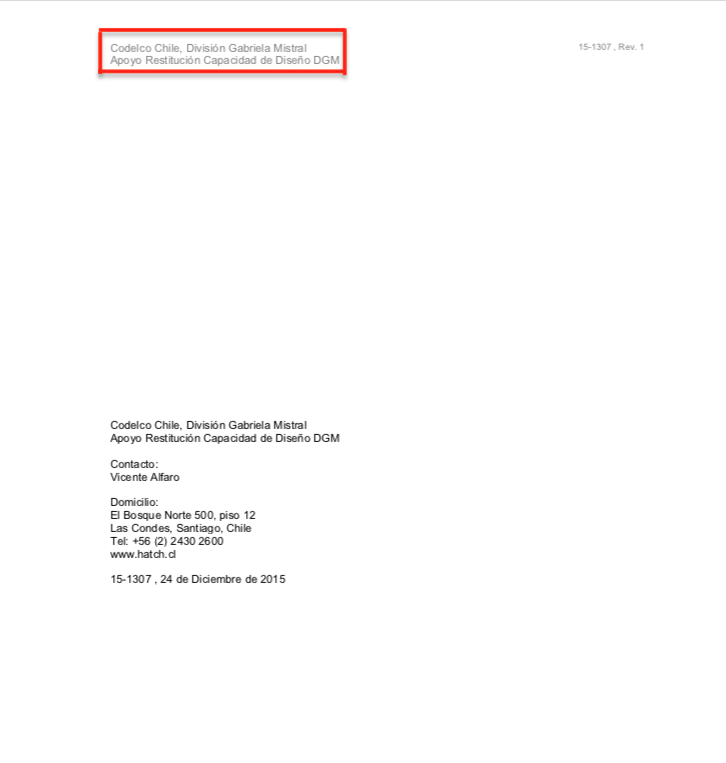
\includegraphics[width=0.8\textwidth]{figures/Header.png}
    \caption{\label{fig:portada_propuesta} Header de una propuesta en general} Fuente: Elaboración Propia.
    \end{figure}
    
    
    
\subsubsection{Análisis exploratorio de datos}
    Una vez preprocesados los textos, es necesario extraer algunas métricas importantes (Ver sección 3.2.2). El corpus a analizar posee un total de 17 documentos en dónde estos han sido clasificados, de manera supervisada, en dos clases: propuestas perdedoras y propuestas ganadoras (Ver tabla: \ref{table:key:_metrics_corpus}).
    
    \begin{table}[H]
    \centering
    \begin{tabular}{|c|c|}
    \hline
    \textbf{Métrica}                                                             & \textbf{Valor} \\ \hline
    \begin{tabular}[c]{@{}c@{}}Número de documentos\\ en la muestra\end{tabular} &   17            \\ \hline
    Número de clases                                                             & 2              \\ \hline
    \end{tabular}
    \caption{\label{table:key:_metrics_corpus} Métricas Corpus}  Fuente: Elaboración Propia 
    \end{table}
    
    Por otro lado, al extraer algunas métricas para cada una de las clases (Ver tabla: \ref{table:key:_metrics}) se puede notar que la mediana de documentos analizados de las propuestas perdedoras es mucho mayor al de las propuestas ganadoras (casi el doble). Además, el número de documentos perdedores a analizar es superior al de los documentos ganadores. 
    
    \begin{table}[H]
    \centering
    \begin{tabular}{|c|c|c|c|}
    \hline
    \textbf{Clase}     & \textbf{Número de propuesta} & \textbf{Mediana de palabras por propuesta} & \textbf{Clientes}\\ \hline
    \textbf{Ganadora}  & 7                            & 111106                                     & 3                 \\ \hline
    \textbf{Perdedora} & 9                            & 213777                                     & 4                 \\ \hline
    \end{tabular}
    \caption{\label{table:key:_metrics} Métricas Claves}  Fuente: Elaboración Propia 
    \end{table}
    
\subsubsection{Transformación de Textos}
    El proceso de transformación de textos depende de cada una de las técnicas que se utilicen (Ver sección 3.2.3). Por ello se describen junto al desarrollo de las técnicas y algoritmos en secciones posteriores . 
    
\subsubsection{Técnicas de Minería de Textos}
    En esta sección se describen en profundidad los experimentos y resultados obtenidos por las técnicas de minería de textos utilizadas en nuestro estudio. 
    
\paragraph{Caracterización de un documento en particular}
\paragraph*{}
    Luego de conocer las métricas claves de nuestro corpus a analizar, también es importante conocer de qué habla un documento en general. La forma más sencilla de realizar este ejercicio es utilizando una nube de palabras (Ver sección 2.5.4.1.1). Para realizar esto se seleccionó un documento al azar ganador y otro documento al azar perdedor obteniendo las visualizaciones (Ver figura \ref{fig:nube_ganadora} y \ref{fig:nube_perdedora} ). 
    
    En general, de ambas nubes de palabras se puede ver que conceptos como proyecto, equipo y diseño son los que más destacan en ambos tipos de propuestas. Además esta visualización nos puede ayudar a tener un acercamiento sobre de que trata un proyecto en particular. Por ejemplo en la propuesta perdedora (Ver figura \ref{fig:nube_perdedora}) se puede ver que se está vendiendo un proyecto de ingeniería básica para el cliente Codelco División Teniente en materias de manejo de materiales. 

\begin{figure}[H]
\centering
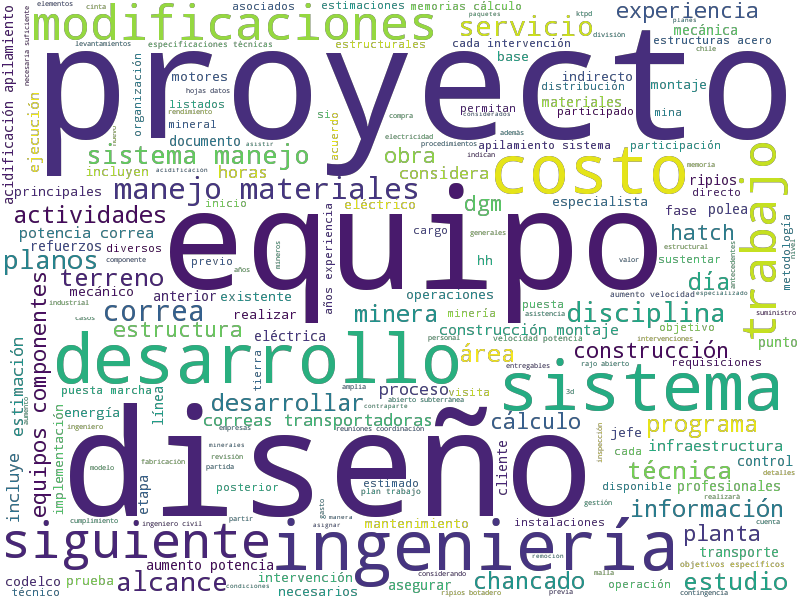
\includegraphics[width=0.8\textwidth]{figures/KeyWords/nube_ganadora.png}
\caption{\label{fig:nube_ganadora} Nube de Palabras de una propuesta ganadora} Fuente: Elaboración Propia.
\end{figure}

\begin{figure}[H]
\centering
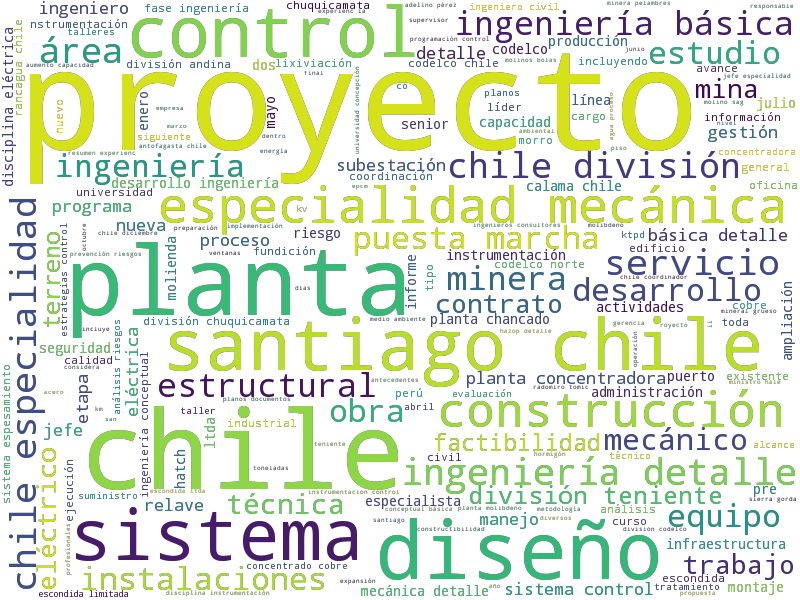
\includegraphics[width=0.8\textwidth]{figures/KeyWords/nube_perdedora.png}
\caption{\label{fig:nube_perdedora} Nube de Palabras de una propuesta perdedora} Fuente: Elaboración Propia.
\end{figure}

\paragraph{Extracción de keywords}
\paragraph*{}
    El objetivo principal del estudio que se está desarrollando, es lograr caracterizar y en lo posible encontrar los patrones que permitan diferenciar a una propuesta ganadora de una perdedora. Teniendo esto en cuenta, se definió que el primer paso que se debía dar era poder entender que hablaba cada una de las propuestas analizadas. Como se vio en la sección anterior, una buena forma de realizar esto era utilizando nubes de palabras pero ¿Será útil realizar esto mismo para un corpus de documentos?, ¿Es viable analizar $n$ nubes de palabras con el fin de entender todo el corpus en cuestión? Las respuestas a todas estas interrogantes anteriores son negativas. Sin embargo, para lograr este objetivo se puede utilizar el proceso de extracción de KeyWords (Ver sección sección 2.5.1) el cual hace uso de n-gramas y nos permitirá caracterizar a un corpus completo de documentos.

\subparagraph{Proceso de extracción de n-gramas y rankeo}
\subparagraph*{}
    Tal como se describe en la sección 2.5.1, para extraer un \textit{keyword} de un documento en particular. Lo primero que se debe realizar es romper el documento en n-gramas. En el caso de esta memoria se decidió analizar al corpus utilizando 2-gramas. Para realizar esto, se puede utilizar el siguiente scrtipt:

    \begin{lstlisting}[language=Python]
    import nltk
    finder = BigramCollocationFinder.from_words(text_tokenized, window_size = 3)
    \end{lstlisting}
    
    Cabe destacar que el script anterior, recibe como parámetro un texto tokenizado, como por ejemplo, el retornado por nuestro normalizador y retorna el texto en 2-gramas.
    
    Una vez realizado este proceso, los 2-gramas (que desde ahora llamaremos bolsas de palabras) deben ser rankeados utilizando alguna métrica. Esto, con el fin de poder encontrar las bolsas de palabras más relevantes dentro del corpus. Para este paso, se utilizaron dos métricas (Ver sección 2.5.1) :
    
    \begin{itemize}
        \item Frecuencia absoluta
        \item Información mutua puntual
    \end{itemize}
    
    Se puede obtener dicho ranking utilizando el siguiente script:
    \begin{lstlisting}[language=Python]
    from nltk.collocations import *
    bigram_measures = nltk.collocations.BigramAssocMeasures()
    #Bow using absolute frequency 
    bow_freq = []
    for k,v in finder.ngram_fd.items():
        bow_freq.append((k,v))
    #Bow using pmi
    bow_pmi = finder.score_ngrams(bigram_measures.pmi)
    \end{lstlisting}
    
     Una vez rankeados todos los documentos, se debió seleccionar un criterio para detectar a las bolsas de palabras \textit{Top} para cada una de las métricas utilizadas, estas bolsas serán los \textit{keywords}. Cuando hablamos de \textit{keywords} nos referimos a las bolsas de palabras más relevantes según la métrica que estemos utilizando dentro de un documento $d$. 
    
    Para realizar este proceso, se decidió seleccionar un umbral para cada una de estas métricas y así las bolsas de palabras que estuvieran sobre este umbral serían \textit{keywords} y en caso contrario serían una bolsa normal. Para seleccionar este umbral, se tomó un documento al azar y se realizó el plot \textit{Número de bolsas de Palabras Vs Frecuencia Absoluta y PMI} respectivamente.
    
    El resultado de este pequeño experimento para la métrica frecuencia absoluta (Ver figura: \ref{fig:BowVsFA} ) fue de 20 apariciones dentro de un documento. Es decir las bolsas de palabras que aparecieran más de 20 veces dentro de un documento se consideran como \textit{keywords}. Esta elección se hizo ya que la idea de encontrar \textit{keywords} era disminuir el número de bolsas a analizar posteriormente y como se puede apreciar en el gráfico (Ver figura \ref{fig:BowVsFA}) la mayoría de las bolsas se concentran en frecuencias entre 0 y 10. Y pocas bolsas son las que tienen una frecuencia superior a 20 , es decir pocas bolsas son las que aparecen mucho en el documento.
    
    \begin{figure}[H]
    \centering
    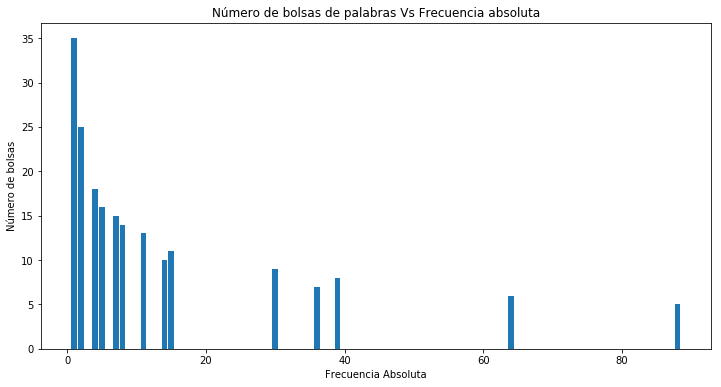
\includegraphics[width=0.8\textwidth]{figures/KeyWords/Umbral_FA.png}
    \caption{\label{fig:BowVsFA} Número de Bolsas Vs Frecuencia Abosluta} Fuente: Elaboración Propia.
    \end{figure}
    
    Por otro lado, el resultado para la métrica de información mutua puntual (Ver figura \ref{fig:BowVsPMI} ) fue bastante desalentador. Como se puede apreciar en la figura existían más de 800 bolsas con un PMI superior a 12 por lo que el objetivo de extraer un número bajo de \textit{keywords} no se cumple usando esta métrica. 
    Considerando lo anterior de aquí en adelante se utilizarán los \textit{keywords} extraídos utilizando la metrica de frecuencia absoluta. 
    
    \begin{figure}[H]
    \centering
    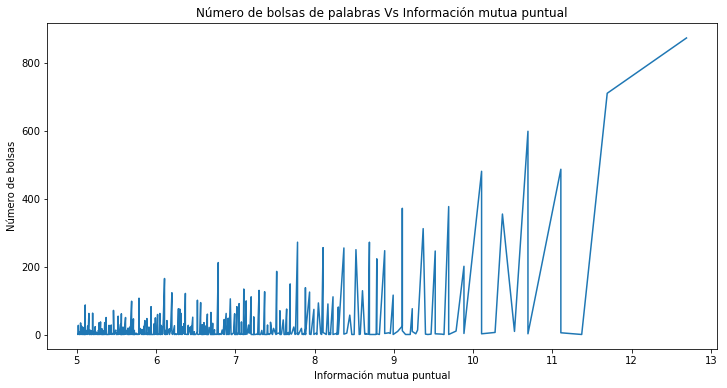
\includegraphics[width=0.8\textwidth]{figures/KeyWords/Umbral_PMI.png}
    \caption{\label{fig:BowVsPMI} Número de Bolsas Vs Información  Mutua Puntual} Fuente: Elaboración Propia.
    \end{figure}

\subparagraph{Comparación de keywords de propuestas ganadoras y perdedoras}
\subparagraph*{}
    Una vez extraídos los \textit{keywords} de todos los documentos tanto ganadores como perdedores, se prosiguió a intentar caracterizar al conjunto de documentos ganadores y al conjunto de documentos perdedores. Para ello se agruparon todos los \textit{keywords}, que al menos aparecieran en dos o más documentos, dentro de las propuestas ganadores y perdedores. Una vez realizado este proceso se obtuvieron los conjuntos $G$ y $P$ que almacenaban los \textit{keywords} para las propuestas ganadores y perdedoras respectivamente. 
    
    Considerando que tenemos dos conjuntos de \textit{keywords}, se optó por realizar operaciones de conjuntos con el fin de encontrar los conceptos comunes entre documentos ganadores y perdedores, además de \textit{keywords} que sólo aparecen en documentos ganadores mas no en perdedores y vice-versa.
    
    A continuación se presentan las operaciones utilizadas y una breve interpretación de sus resultados:
    
    \begin{itemize}
        \item $G \cap P$: La intersección entre los keywords ganadores y perdedores (Ver tabla: \ref{table:Conceptos_comunes}) es interpretada como el conjunto de elementos básicos dentro de cualquier propuesta. 
        
        \begin{table}[H]
        \centering
        \begin{tabular}{|c|c|}
        \hline
        \textbf{Concepto 1} & \textbf{Concepto 2} \\ \hline
        Años                & Experiencia         \\ \hline
        Desarrollo          & Ingeniería          \\ \hline
        Específicaciones    & Técnicas            \\ \hline
        Gestión             & Cálidad             \\ \hline
        Ingeniería          & Básica              \\ \hline
        Ingeniería          & Detalles            \\ \hline
        Lider               & Disciplina          \\ \hline
        Plan                & Cálidad             \\ \hline
        Prevencion          & Riesgos             \\ \hline
        Salud               & Ocupacional         \\ \hline
        Seguirdad           & Salud               \\ \hline
        Sistema             & Gestión             \\ \hline
        \end{tabular}
        \caption{\label{table:Conceptos_comunes} Conceptos comunes en cualquier propuesta} Fuente: Elaboración Propia
        \end{table}
        
        De aquí se puede apreciar que elementos como ``Gestión de Cálidad'', ``Prevención de Riesgos'' , ``Sistemas de Gestión'' son temas tratados en la mayoría de las propuestas de la compañía. Por otro lado, adjetivos positivos para calificar a la compañía como \textit{``Años de Experiencia''}, \textit{``Líder Disciplina''} también son utilizados para cualquier propuesta.
        
        \item $G - P$: La diferencia entre los \textit{keywords} ganadores y perdedores puede ser interpretada como los elementos que fueron resaltados en las propuestas ganadoras mas no en las perdedoras (Ver tabla: \ref{table:Conceptos_con_valor}). Esto quiere decir que podrían ser elementos que entregaron valor a la propuesta para hacerla ganadora.
        
        \begin{table}[H]
        \centering
        \begin{tabular}{|c|c|}
        \hline
        \textbf{Concepto 1} & \textbf{Concepto 2} \\ \hline
        Calidad             & Hatch               \\ \hline
        Cliente             & Hatch               \\ \hline
        Control             & Documentos          \\ \hline
        Coordinador         & Calidad             \\ \hline
        Ejecución           & Servicios           \\ \hline
        Estándar            & Cuidado             \\ \hline
        Evaluación          & Todas               \\ \hline
        Medio               & Ambiente            \\ \hline
        Obras               & Anexas              \\ \hline
        Modelo              & Dinámico            \\ \hline
        Ingeniería          & Cierre              \\ \hline
        \end{tabular}
        \caption{\label{table:Conceptos_con_valor} Conceptos que entregan valor a una propuesta} Fuente: Elaboración Propia
        \end{table}
        
        Aquí se puede apreciar cómo por ejemplo, vincular los conceptos Clientes, Calidad y Hatch tuvo resultados positivos en el resultado de algunas propuestas. Además también se puede ver cómo hablar sobre prácticas que realiza la compañía sobre ciertos procesos, traen un buen impacto en el resultado final de una propuesta. Como por ejemplo \textit{''Estándar Cuidado``}, \textit{''Evaluación Todas``}, \textit{''Coordinador Calidad``}, \textit{''Control de Documentos``}.
        
        \item $P - G$: La diferencia entre los \textit{keywords} perdedores y ganadores (Ver tabla: \ref{table:Conceptos_sin_valor}) puede ser interpretada como los elementos que fueron resaltados en las propuestas perdedoras mas no en las ganadoras. Esto quiere decir que es probable que estos \textit{keywords} no ayudaron a ganar la propuesta.
        
        \begin{table}[H]
        \centering
        \begin{tabular}{|c|c|}
        \hline
        \textbf{Concepto 1} & \textbf{Concepto 2} \\ \hline
        Civil               & Estructural         \\ \hline
        Compañía            & Minera              \\ \hline
        Disciplina          & Mecánica            \\ \hline
        Diseño              & Planos              \\ \hline
        Ingenieros          & Consultores         \\ \hline
        Ingeniería          & Conceptual          \\ \hline
        Jefe                & Disciplina          \\ \hline
        Manejo              & Materiales          \\ \hline
        Puesta              & Marcha              \\ \hline
        \end{tabular}
        \caption{\label{table:Conceptos_sin_valor} Conceptos importantes en propuestas perdedoras pero no en ganadoras} Fuente: Elaboración Propia
        \end{table}
    \end{itemize}
    Si bien se le podría otorgar una connotación negativa a muchos de estos conceptos, en la práctica esto es imposible de hacer. Esto se debe a que, por ejemplo, los conceptos ``Ingeniería Conceptual'', ``Civil Estructural'' y ''Diseño de Planos`` son disciplinas en sí mismas por lo que claramente estarán siempre en una propuesta de Construcción, por ejemplo. Es por lo anterior que este conjunto de \textit{keywords} no entrega información utilizable.
\subparagraph{Análisis temporal de keywords comunes para una propuesta} 
\subparagraph*{}
    Del análisis anterior, se extrajo una lista de \textit{keywords} que fueron identificados como elementos básicos dentro de una propuesta. Una pregunta interesante de responder sería ¿Cómo interactúan estos \textit{keywords} a lo largo de todos los documentos analizados? Para responder a esto podemos hacer uso de un gráfico de dispersión léxica (Ver sección 2.5.4.1.1) .
    
    Antes de explicar los resultados encontrados, es necesario detallar el modo en cómo se utilizó el gráfico de dispersión léxica. En general, un gráfico de dispersión léxica se utiliza para ver cómo se comporta una serie de conceptos a lo largo de un documento. En nuestro caso como se desea analizar el comportamiento de \textit{keywords} en un conjunto de documentos, se realizó una pequeña modificación a la visualización original. Esta consiste en analizar un único concepto por gráfico. Para lograr esto, en el eje Y en vez de escribir los conceptos a analizar, se escribieron el nombre de los documentos analizados. Por otro lado, el eje X sigue mostrando la temporalidad del texto en su forma relativa (posición de la palabra dividida en el largo del documento), mientras que en el título del gráfico se puede ver qué \textit{keyword} se está analizando. Con esto se pudo comparar cómo un único concepto era tratado en distintos documentos tanto ganadores como perdedores.
    
    \begin{lstlisting}[language=Python]
    def dispersion_plot_1_token(documents,token,color="blue",y_axis="id"):
        points = []
        for y in range(len(documents)):
            for x in range(len(documents[y]["Tokens_bigram"])):
                if (documents[y]["Tokens_bigram"][x] == token):
                    points.append(((x*100)/len(documents[y]["Tokens_bigram"]),y))
            if points:
                x,y = list(zip(*points))
            else:
                x = y = ()
        yticks = [i["id"] for i in documents]
        if (y_axis != "id"):
            yticks = [i["Proyecto"][0:45] for i in documents]
        fig, ax = plt.subplots(figsize=(12,6))
        plt.plot(x, y, "|", color=color, scalex=.1)
        plt.tick_params(
            axis='x', which='both', bottom='off', labelbottom='off'
        )
        plt.xlabel('Temporalidad del texto')
        plt.yticks(list(range(len(documents))),yticks)
        plt.ylim(-1, (len(documents)))
        plt.title("Análisis de dispersión léxica para " + str(token) + " en propuestas " + documents[0]["Estado"]+"s")
        plt.savefig("img/DispersionPlot_"+str(token)+"_"+color,bbox_inches='tight')
        plt.show()
    \end{lstlisting}
    
    La función anterior recibe como parámetros al conjunto de documentos, en el formato \textit{json} definido en el capítulo anterior y el token a analizar. Además se da la opción de seleccionar el color de las barras del gráfico de dispersión léxica.
    
    A continuación, se describen los hallazgos más importantes que se pudieron recabar realizando este análisis. Cabe destacar que muchos \textit{keywords}, si bien fueron analizados, no se encontró ningún patrón relevante por lo que no se añadió a la discusión.
    
    \begin{itemize}
        \item \textbf{Salud Ocupacional}: Como se puede apreciar en 3 de las propuestas ganadoras (Ver figura: \ref{fig:SO_Win} ) hay una sección completa dedicada a aspectos de salud ocupacional. Sin embargo es difícil dar una connotación positiva a esto, ya que en las 4 propuestas restantes el concepto se menciona en puntos específicos del texto e incluso en algunos no se llega a nombrar. Por otro lado, en las propuestas perdedoras (Ver figura: \ref{fig:SO_Loss}) se puede apreciar que varios documentos poseen una sección dedicada a temas de salud ocupacional tal como pasaba en algunos documentos ganadores. Sin embargo hay una diferencia sustancial entre estos documentos y los ganadores y es que en los documentos ganadores, se puede ver que el concepto es tratado desde el comienzo en forma paulatina hasta que llega a una sección completamente dedicada a él. En cambio, en los documentos perdedores que poseen una sección dedicada a salud ocupacional se puede apreciar cómo el concepto es tratado a lo largo de todo el texto, con incluso secciones separadas tanto al inicio como el final (posibles anexos). 
        
        \begin{figure}[H]
        \centering
        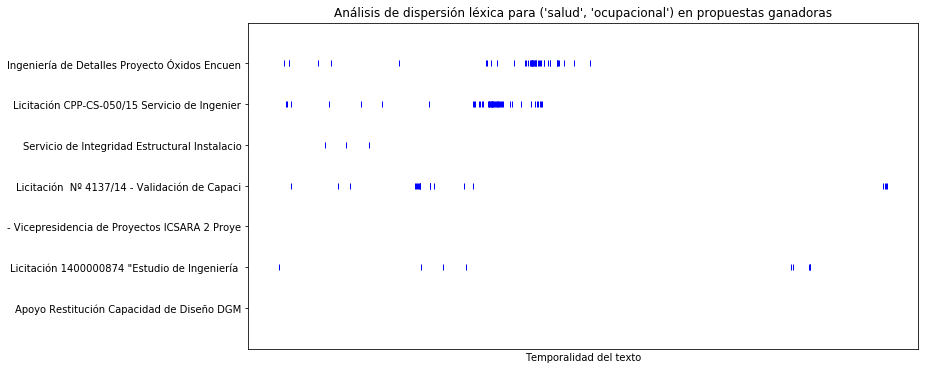
\includegraphics[width=0.8\textwidth]{figures/KeyWords/DispersionPlot_(salud,ocupacional)_blue.png}
        \caption{\label{fig:SO_Win} Dispersión Léxica del concepto Salud Ocupacional en propuestas ganadoras} Fuente: Elaboración Propia.
        \end{figure}
            
        \begin{figure}[H]
        \centering
        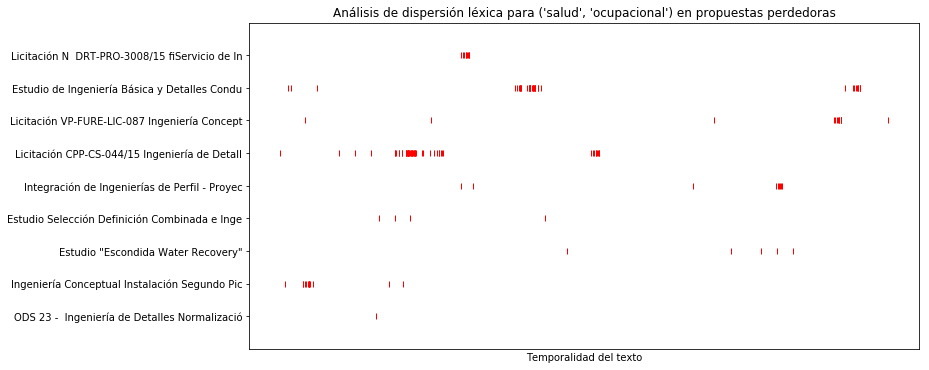
\includegraphics[width=0.8\textwidth]{figures/KeyWords/DispersionPlot_(salud,ocupacional)_red.png}
        \caption{\label{fig:SO_Loss} Dispersión Léxica del concepto Salud Ocupacional en propuestas perdedoras} Fuente: Elaboración Propia.
        \end{figure}
        
        \item \textbf{Gestión de Calidad}: Como se puede apreciar en general, las propuestas perdedoras (Ver figura: \ref{fig:GC_Loss}) poseen un apartado especial sobre Gestión de Calidad. Sin embargo, este concepto no está en un lugar específico para todos los documentos, por ejemplo se puede ver que en el proyecto \textit{Estudio ``Escondida Water Recovery''} la sección del concepto estudiado se encuentra al final del documento, mientras que en el resto de documentos analizados ésta se encuentra más al inicio. Por otro lado, para los documentos ganadores, (Ver figura: \ref{fig:GC_Win} ) se puede apreciar que si bien ciertos documentos poseen una sección de Gestión de Calidad existen muchos que no la tienen. Además tal como ocurre en las propuestas perdedoras, no existe un lugar específico en donde tratar este concepto dentro de los documentos, por lo que no podemos darle connotaciones negativas ni positivas al lugar donde se utiliza el concepto.
        
        \begin{figure}[H]
        \centering
        \includegraphics[width=0.8\textwidth]{figures/KeyWords/DispersionPlot_(gestión,calidad)_blue.png}
        \caption{\label{fig:GC_Win} Dispersión Léxica del concepto Gestión de Calidad en propuestas ganadoras} Fuente: Elaboración Propia.
        \end{figure}
        
        \begin{figure}[H]
        \centering
        \includegraphics[width=0.8\textwidth]{figures/KeyWords/DispersionPlot_(gestión,calidad)_red.png}
        \caption{\label{fig:GC_Loss} Dispersión Léxica del concepto Gestión de Calidad en propuestas ganadoras} Fuente: Elaboración Propia.
        \end{figure}
    \end{itemize}

    \paragraph{Modelamiento de tópicos}
    \paragraph*{}
    El siguiente experimento que se debe realizar, es el de modelamiento de tópicos (Ver sección 3.2.4.2). La idea ahora es analizar a los documentos considerando los temas latentes que tratan éstos.  
    
    \subparagraph{Transformación de textos}
    \subparagraph*{}
    Como en todo algoritmo de minería de textos, antes de poder ser utilizado es necesario efectuar una transformación a los textos de tal forma que puedan ser interpretados por la técnica a utilizar. En nuestro caso, el algoritmo LDA recibe como parámetros un diccionario de palabras de la forma: \textit{(palabra , frecuencia)} con el fin de poder ponderar la importancia de cada palabra dentro de un documento en específico. El resultado para un documento en particular se puede apreciar a continuación:
    
    \begin{lstlisting}[language=Python]
    [[(0, 1), (1, 2), (2, 1), (3, 1), (4, 1), (5, 1), (6, 5), (7, 1), (8, 1), (9, 2), (10, 1), (11, 1), (12, 1), (13, 1), (14, 1), (15, 1), (16, 1), (17, 1), (18, 1), (19, 1), (20, 1), (21, 1), (22, 2), (23, 1), (24, 1), (25, 1), (26, 1), (27, 1), (28, 1), (29, 1), (30, 1), (31, 1), (32, 1), (33, 1), (34, 1), (35, 1), (36, 1), (37, 1), (38, 1), (39, 1), (40, 1), (41, 1), (42, 1), (43, 1), (44, 1), (45, 1), (46, 1), (47, 1), (48, 1), (49, 1), (50, 1)]]
    \end{lstlisting}
    
    \subparagraph{Construcción y parametrización del  modelo}
    \subparagraph*{}
    
    Como se describió en las secciones anteriores, para la construcción de un modelo LDA es necesaria la elección de 3 parámetros: \textit{Alfa}, \textit{Beta} y $k$ (número de temas). Los hiper-parámetros alfa y beta, son relacionados a la variabilidad buscada en los temas y documentos analizados, por lo que en general poseen valores estándares seleccionados. Por otro lado, seleccionar el número $k$ adecuado de temas a modelar es una tarea que merece un tratamiento un poco más elaborado. 
    
    Para poder hacer una buena elección del número $k$ de temas a modelar, se puede utilizar el valor de coherencia para un modelo LDA con un $k$ en particular. Dentro de esta memoria, se crearon modelos para distintos valores de $k$ (ver figura \ref{fig:Coherence}) y se calculó el número de coherencia para cada uno de ellos. En general se puede apreciar que el índice de coherencia aumenta hasta un $k=8$ y luego de este valor el índice comienza a descender por lo que se utilizará este valor para crear el modelo a analizar.
    
    \begin{figure}[h!]
        \centering
        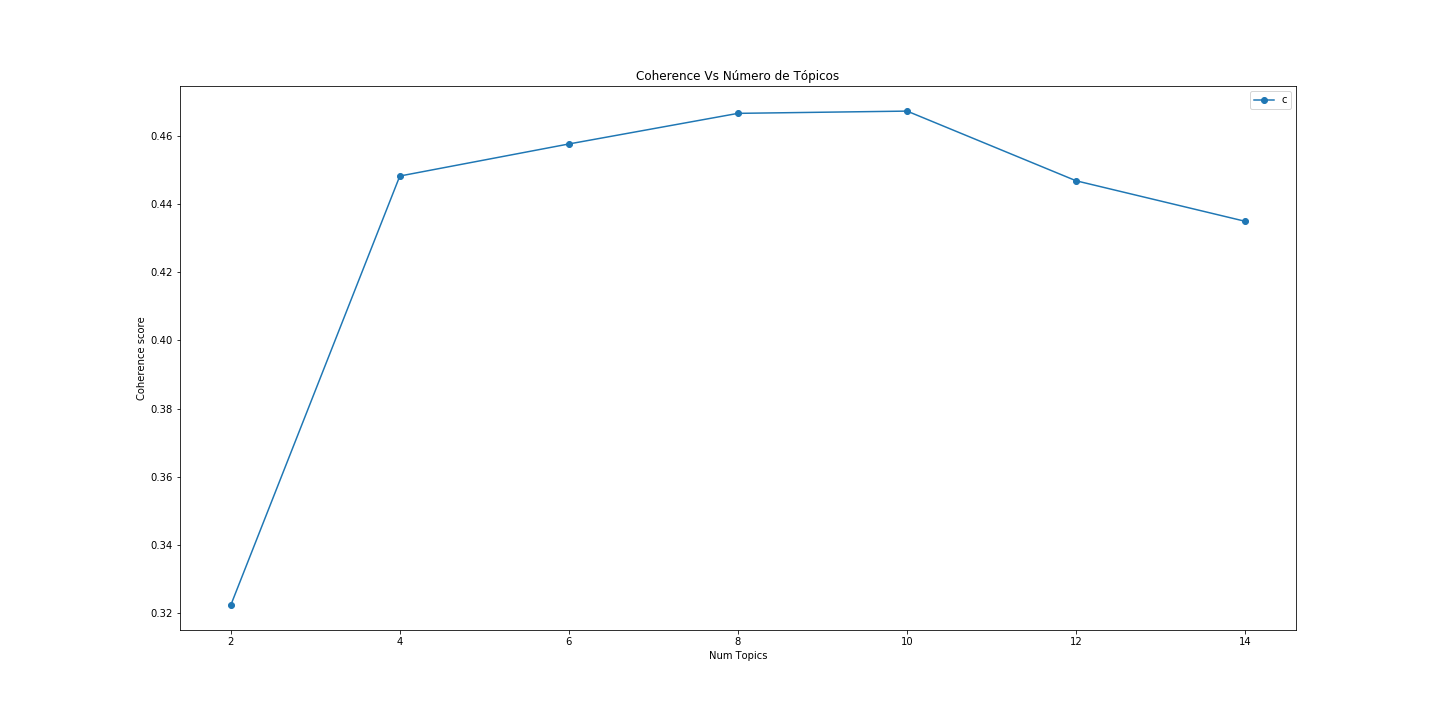
\includegraphics[width=0.8\textwidth]{figures/LDA/Coherence.png}
        \caption{\label{fig:Coherence} Índice de Coherencia Vs Número de Tópicos} Fuente: Elaboración Propia.
    \end{figure}
    
    Una vez creado el modelo, se puede comenzar a ver sus resultados. En este caso se encontraron 8 temas y como se sabe, se puede visualizar cada uno de ellos como una distribución de palabras. A continuación, se puede ver en detalle la composición de cada uno de los temas encontrados: 
    
    \begin{itemize}
        \item \textbf{Tema 0}: 0.011*jefe + 0.010*obras + 0.010*relaves + 0.007*seguridad + 0.007*aguas + 0.007*sistema + 0.007*diseño + 0.007*estudio + 0.007*conducción + 0.006*ambiental
        
        \item \textbf{Tema 1}: 0.013*parte + 0.012*contrato + 0.011*cliente + 0.011*servicios + 0.007*ser + 0.006*información + 0.006*codelco + 0.006*siguientes + 0.006*cualquier + 0.006*acuerdo
        
        \item \textbf{Tema 2}: 0.024*planta + 0.017*cobre + 0.012*prefactibilidad + 0.012*estudio + 0.011*lixiviación + 0.011*análisis + 0.010*control + 0.009*operación + 0.008*caso + 0.007*nacional

        \item \textbf{Tema 3}: 0.015*process + 0.012*fundición + 0.010*smelter + 0.009*copper + 0.009*planta + 0.009*project + 0.008*plant + 0.008*engineer + 0.008*chuquicamata + 0.008*procesos

        \item \textbf{Tema 4}: 0.018*relaves + 0.012*andina + 0.010*obras + 0.009*estudio + 0.008*agua + 0.008*región + 0.007*análisis + 0.006*etapa + 0.006*aguas + 0.006*tranque
        
        \item \textbf{Tema 5}: 0.011*seguridad + 0.011*sistema + 0.011*chancado + 0.010*diseño + 0.010*gestión + 0.009*construcción + 0.008*planos + 0.008*ejecución + 0.007*información + 0.007*control
        
        \item \textbf{Tema 6}: 0.017*planta + 0.011*sistema + 0.011*minera + 0.010*diseño + 0.009*control + 0.008*disciplina + 0.008*detalles + 0.008*equipos + 0.008*codelco + 0.007*manejo
        
        \item \textbf{Tema 7}: 0.023*calidad + 0.011*control + 0.011*codelco + 0.011*desarrollo + 0.010*gestión + 0.009*servicio + 0.008*procesos + 0.007*documentos + 0.007*cumplimiento + 0.007*procedimientos
    \end{itemize}
    
    \newpage
    
    \subparagraph{Interpretación del modelo}
    \subparagraph*{}
    Una vez obtenido el modelo LDA comienza la parte más compleja de éste, la cual es, interpretar los resultados encontrados. Lo primero que se debe realizar cuando se obtienen los temas subyacentes al corpus estudiado, es intentar asignarles algún nombre fácil de identificar (Ver tabla: \ref{table:Topics_Name} ). En nuestro caso, se logró asignarle el nombre a cada uno de los temas con ayuda de expertos en el dominio.
    
    \begin{table}[H]
    \centering
    \begin{tabular}{|c|c|}
    \hline
    \textbf{Tema} & \textbf{Nombre}               \\ \hline
    0             & Seguridad e Impacto Ambiental \\ \hline
    1             & Atención al cliente           \\ \hline
    2             & Cobre                          \\ \hline
    3             & Fundición                     \\ \hline
    4             & Tratamiento de Relaves        \\ \hline
    5             & Construcción        \\ \hline
    6             & Minería                              \\ \hline
    7             & Gestión de Calidad            \\ \hline
    \end{tabular}
    \caption{\label{table:Topics_Name} Nombres para Tópicos encontrados} Fuente: Elaboración Propia
    \end{table}
    
    Una forma de interpretar los resultados de LDA, es asignar a cada documento su tópico más representativo. Para realizar esto, simplemente se asigna el documento al tópico cuya probabilidad es más alta dentro de su propia distribución de probabilidades. En nuestro caso, se puede apreciar cómo la mayoría de los documentos analizados (Ver figura: \ref{fig:FreqperTopic}) hablan en su mayoría del tópico Gestión de Calidad. Además, también se puede apreciar cómo sólo un documento pertenece a los tópicos Fundición y Cobre respectivamente.
    
    \begin{figure}[H]
        \centering
        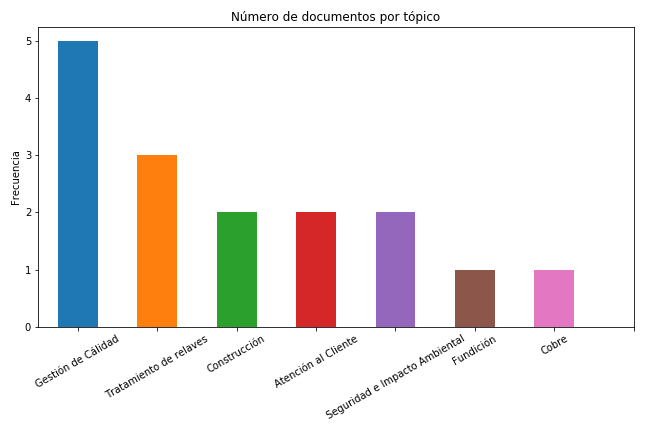
\includegraphics[width=0.8\textwidth]{figures/LDA/documents_per_topic.png}
        \caption{\label{fig:FreqperTopic} Frecuencia de documentos por tópico} Fuente: Elaboración Propia.
    \end{figure}
    
    El mismo análisis efectuado anteriormente, se puede realizar un poco más fino, esta vez viendo cuál es la probabilidad de cada documento de pertenecer a cierto tópico. Para realizar esto se creó un gráfico de barras para cada uno de los 8 tópicos (Ver figura: \ref{fig:TopicPerDoc}), en donde las barras muestran la probabilidad de cada documento de pertenecer al tópico $i$. Para ver una diferencia entre documentos ganadores y perdedores, se optó por pintar de azul las propuestas ganadores y de rojo las perdedoras.
    
    \begin{figure}[h!]
        \centering
        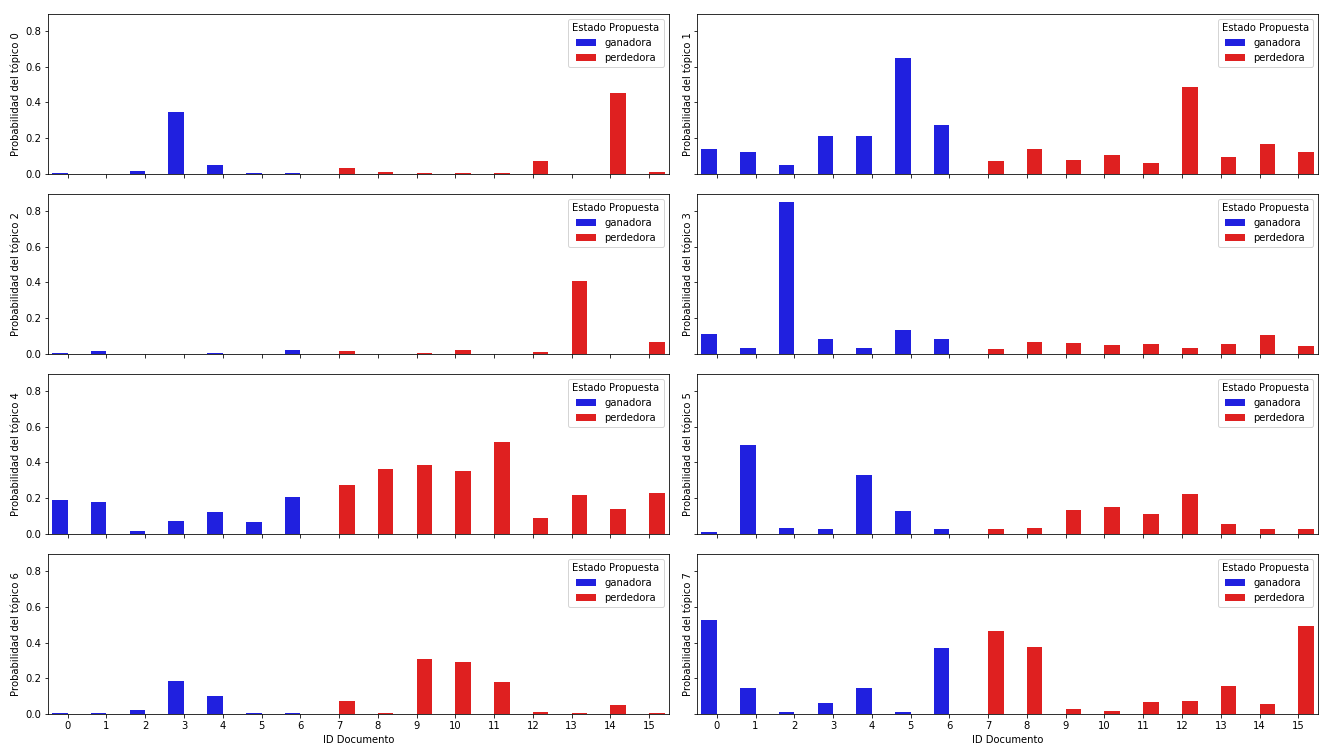
\includegraphics[width=1\textwidth]{figures/LDA/distribution.png}
        \caption{\label{fig:TopicPerDoc} Probabilidad de documentos de pertenecer al tópico $i$} Fuente: Elaboración Propia.
    \end{figure}
    
    Analizando la visualización, se puede apreciar que existen ciertos tópicos que son tratados en sólo ciertos documentos, éste es el caso del tópico 2 (\textit{Cobre}), por ejemplo, el cual es tratado en un 40\% dentro de un sólo documento y no pasando el 10\% en los documentos restantes.

    Otra cosa interesante que podemos extraer de esta visualización, es que en general todos los documentos tratan algo sobre el tópico 4 llamado Tratamiento de Relaves. De hecho, se puede apreciar que en los documentos perdedores, la importancia para este tópico es superior al 30\%, en 5 de los documentos estudiados. Esto quiere decir, que la mayoría de los documentos perdedores que se han analizado hablan mucho sobre este tema.
    
    Como se sabía del punto anterior los tópicos 3 ``Fundición'' y 2 ``Cobre'', tienen sólo un documento que habla en su mayoría de ellos. Sin embargo, se puede apreciar que el documento que habla más del tópico 3, lo hace en un 80\%. Este documento es probablemente un outlier dentro de la muestra.
    
\paragraph{Clustering usando el resultado de Modelamiento de Tópicos}
\paragraph*{}
    Como se habló al inicio de esta sección, la distribución de probabilidades de cada documento de pertenecer a cierto tópico puede ser tratada como la identificación de este documento o incluso como \textit{features} de este mismo. Es por ello que ahora se utilizarán estas características, con el fin de realizar un análisis de \textit{clustering}.
    
\subparagraph{Distancia entre documentos}
\subparagraph*{}
    En primer lugar, antes de realizar el análisis de clusters, se puede visualizar las distancias entre todos los documentos. Esto sirve, para tener una idea de posibles outliers o clusters que se podrían formar con los datos. Para realizar esto, se decidió utilizar la distancia de Jensen-Shannon, para construir una matriz de distancias entre todos los documentos (Ver figura \ref{fig:DistanceMatrix}). Esta elección se hizo debido a que la distancia de Jensen Shannon, es la única construida para medir distancias entre distribuciones de probabilidades.
    
    \begin{figure}[H]
        \centering
        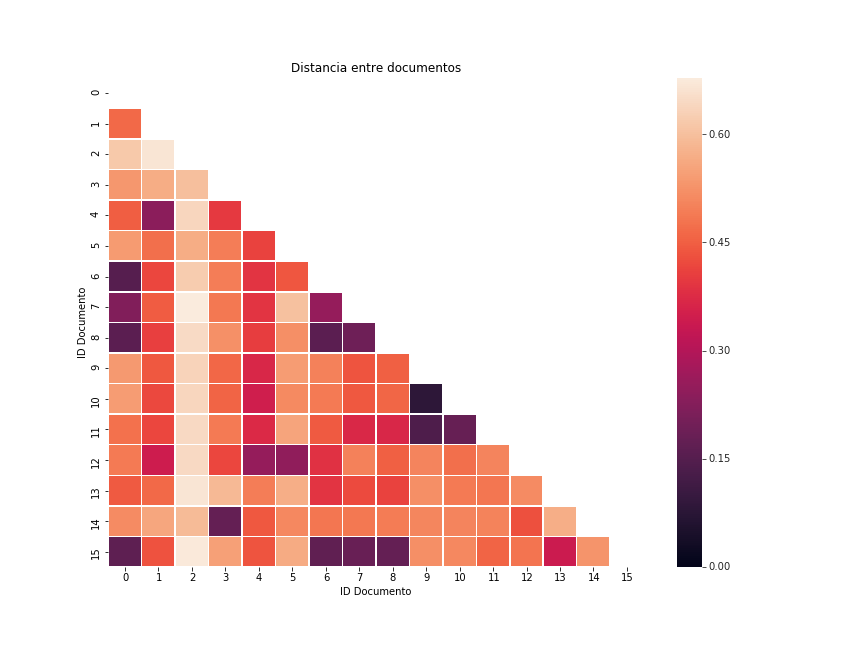
\includegraphics[width=1\textwidth]{figures/Clustering/distancia.png}
        \caption{\label{fig:DistanceMatrix} Matriz de distancia de documentos} Fuente: Elaboración Propia.
    \end{figure}
    
    De esta visualización, se pueden extraer algunas conclusiones:
    \begin{itemize}
        \item El documento 2, es un outlier debido a que se encuentra alejado de todos los documentos. De hecho como habíamos detectado antes, es el único que tiene como tópico principal a ``Fundición''. 
        \item El documento 0, está muy cercano a los documentos 6,7,8 y 15. Cuyo tópico dominante es Gestión de calidad.
    \end{itemize}
    Una vez realizado este análisis, se procederá a aplicar algoritmos de \textit{clustering} para afirmar las conclusiones recién extraídas.
    
    \newpage
    
\subparagraph{Selección del modelo}
\subparagraph*{}
    Para realizar este análisis, se utilizaron dos técnicas de \textit{clustering}: 
    \begin{itemize}
        \item \textbf{K-Means}: Posee como parámetro el número $k$ de \textit{clusters} a encontrar.
        \item \textbf{Jerárquico Aglomerativo}: Posee como parámetros el número $k$ de \textit{clusters} a encontrar, una métrica de distancias y un criterio de enlaces entre \textit{cluster}. 
    \end{itemize}
    Para cada uno de estos algoritmos, se variaron todos sus parámetros construyendo 9 modelos, uno por cada configuración, variando $k$ entre 2 y 9. Para el caso del algoritmo de \textit{clustering} jerárquico aglomerativo se utilizarón las métricas de distancia: Euclidiana, Jensen-Shannon y de Manhattan (Ver sección 2.5.3). Además como criterios de enlace se utilizó: complete, average y single (Ver sección 2.5.3.1). 
    
    Una vez construidos todos los modelos, se procedió a calcular el índice de Silhouette para cada uno de ellos (Ver figuras: \ref{fig:aglomerative_silhoutte} y \ref{fig:k-means_silhoutte}). En general se puede apreciar que los mejores resultados se obtienen con $k=7$. De hecho se obtienen los mejores índices de Silhoutte con $k=7$ para K-means y \textit{clustering} aglomerativo con las distancias de manhattan y euclideana usando todos los criterios de enlace.

     \begin{figure}[H]
        \centering
        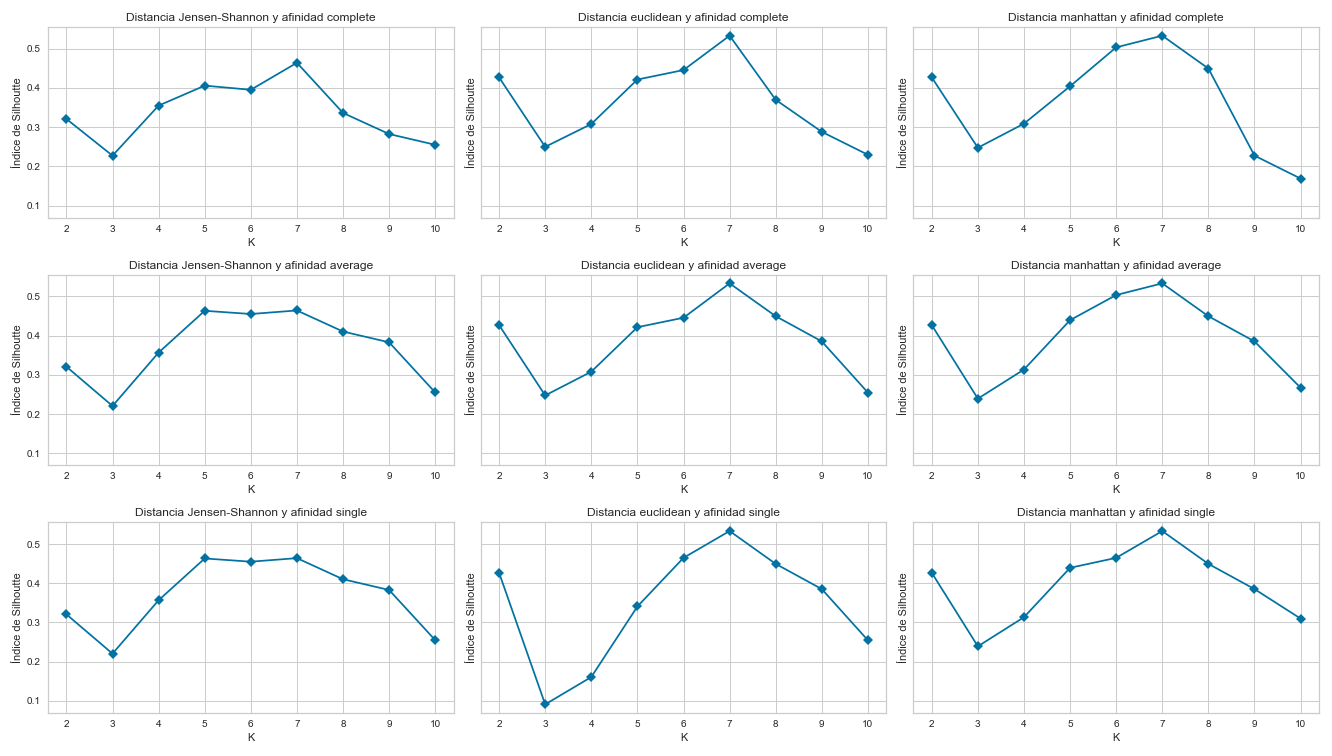
\includegraphics[width=1\textwidth]{figures/Clustering/aglomerative_clustering.png}
        \caption{\label{fig:aglomerative_silhoutte} Evaluación de modelos creados con clustering aglomerativo} Fuente: Elaboración Propia.
    \end{figure}
    
    \begin{figure}[H]
        \centering
        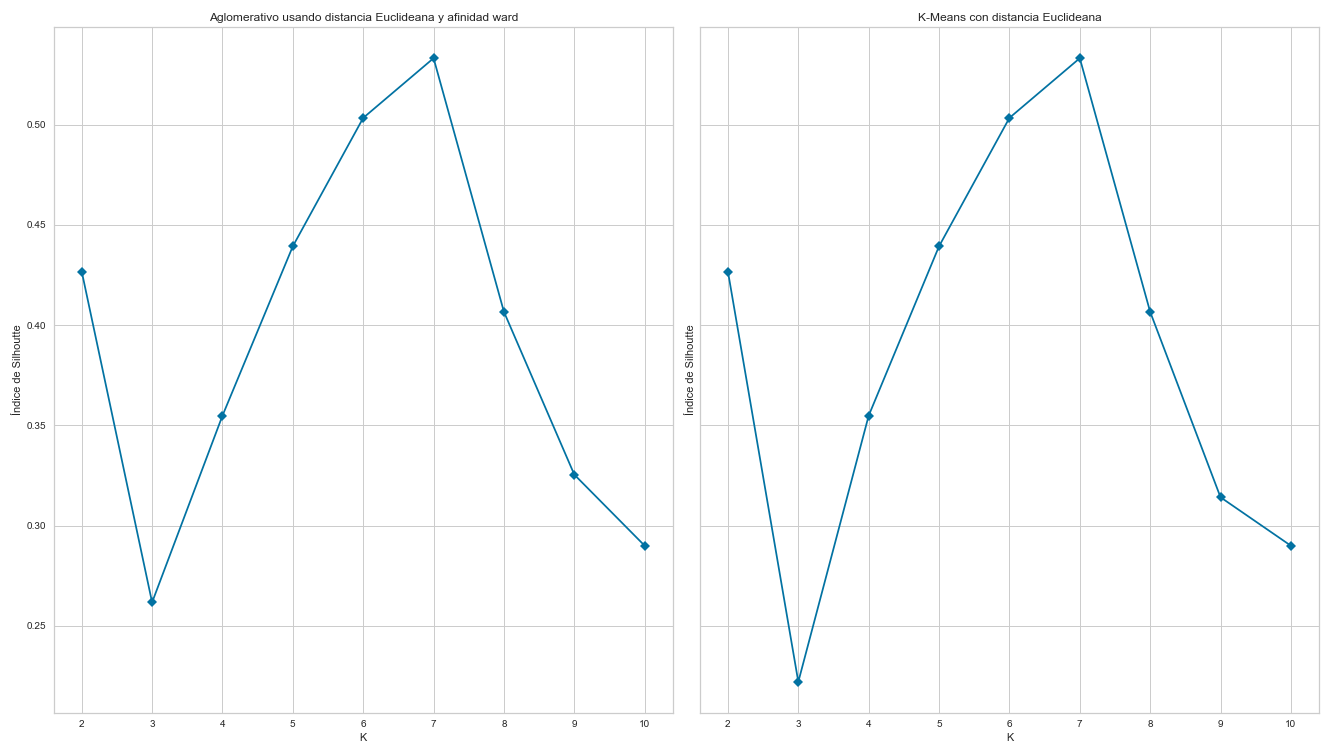
\includegraphics[width=1\textwidth]{figures/Clustering/k-means.png}
        \caption{\label{fig:k-means_silhoutte} Evaluación de modelos creados con clustering aglomerativo y K-Means} Fuente: Elaboración Propia.
    \end{figure}
    
    Considerando lo anterior, se analizó la conformación de los \textit{clusters} con $k=7$ para cada uno de los algoritmos estudiados (Ver tabla: \ref{table:Cluster_Etiquetas}). Como se puede apreciar, los \textit{clusters} encontrados por los dos algoritmos son idénticos a los grupos de temas encontrados por LDA, esto considerando al tópico más relevante como aquel que posee la mayor probabilidad de ocurrencia en el documento. Por ende, pese a que el índice de Silhoutte para la configuración con $k=7$ es el óptimo, no consideraremos este modelo. 
    \begin{table}[H]
    \centering
\begin{tabular}{|c|c|c|c|c|}
\hline
   & Tópico más relevante & id Documento & K-Means & Aglomerativo \\ \hline
0  & 7                    & 15-1307      & 2       & 1            \\ \hline
1  & 5                    & 15-3939      & 5       & 2            \\ \hline
2  & 3                    & 14-5143      & 3       & 3            \\ \hline
3  & 0                    & 14-5115      & 4       & 4            \\ \hline
4  & 5                    & 15-4316      & 5       & 2            \\ \hline
5  & 1                    & 15-3732      & 0       & 0            \\ \hline
6  & 7                    & 14-5142      & 2       & 1            \\ \hline
7  & 7                    & 14-5040      & 2       & 1            \\ \hline
8  & 7                    & 14-4984      & 2       & 1            \\ \hline
9  & 4                    & 14-4770      & 1       & 6            \\ \hline
10 & 4                    & 14-5116      & 1       & 6            \\ \hline
11 & 4                    & 14-5205      & 1       & 6            \\ \hline
12 & 1                    & 15-4448      & 0       & 0            \\ \hline
13 & 2                    & 15-4591      & 6       & 5            \\ \hline
14 & 0                    & 15-4400      & 4       & 4            \\ \hline
15 & 7                    & 15-5050      & 2       & 1            \\ \hline
\end{tabular}
    \caption{\label{table:Cluster_Etiquetas} Resumen Etiquetas de documentos para $k=7$} Fuente: Elaboración Propia
\end{table}
    
   Como la configuración utilizada con $k=7$ no fue la deseada, se decidió analizar las configuraciones encontradas para $k=6$ (Ver tabla: \ref{table:Cluster_Etiquetas_6} ) y $k=5$ (Ver tabla: \ref{table:Cluster_Etiquetas_5} ). 
   
   Para el caso de $k=6$, los documentos cuyo tópico dominante es el $7$, ``Gestión de calidad'', y el $2$, ``Cobre'', se unieron en un único \textit{cluster}. Por otro lado para $k=5$ además del nuevo \textit{cluster}, formado para $k=6$, los documentos cuyo tópico dominante era el $1$, ``Atención al cliente'' y el $5$ ``Construcción'' también se unieron en un único \textit{cluster}.
   
    \begin{table}[H]
    \centering
    \begin{tabular}{|c|c|c|c|}
    \hline
    Tópico más relevante & id Documento & K-Means & Aglomerativo \\ \hline
    0                    & 14-5115      & 4       & 4            \\ \hline
    0                    & 15-4400      & 4       & 4            \\ \hline
    1                    & 15-3732      & 0       & 2            \\ \hline
    1                    & 15-4448      & 0       & 2            \\ \hline
    2                    & 15-4591      & 2       & 0            \\ \hline
    3                    & 14-5143      & 3       & 3            \\ \hline
    4                    & 14-4770      & 1       & 1            \\ \hline
    4                    & 14-5116      & 1       & 1            \\ \hline
    4                    & 14-5205      & 1       & 1            \\ \hline
    5                    & 15-3939      & 5       & 5            \\ \hline
    5                    & 15-4316      & 5       & 5            \\ \hline
    7                    & 15-1307      & 2       & 0            \\ \hline
    7                    & 14-5142      & 2       & 0            \\ \hline
    7                    & 14-5040      & 2       & 0            \\ \hline
    7                    & 14-4984      & 2       & 0            \\ \hline
    7                    & 15-5050      & 2       & 0            \\ \hline
    \end{tabular}
    \caption{\label{table:Cluster_Etiquetas_6} Resumen Etiquetas de documentos para $k=6$} Fuente: Elaboración Propia
    \end{table}
    
    \begin{table}[H]
    \centering
\begin{tabular}{|c|c|c|c|}
\hline
Tópico más relevante & id Documento & K-Means & Aglomerativo \\ \hline
0                    & 14-5115      & 4       & 4            \\ \hline
0                    & 15-4400      & 4       & 4            \\ \hline
1                    & 15-3732      & 0       & 0            \\ \hline
1                    & 15-4448      & 0       & 0            \\ \hline
2                    & 15-4591      & 2       & 2            \\ \hline
3                    & 14-5143      & 3       & 3            \\ \hline
4                    & 14-4770      & 1       & 1            \\ \hline
4                    & 14-5116      & 1       & 1            \\ \hline
4                    & 14-5205      & 1       & 1            \\ \hline
5                    & 15-3939      & 0       & 0            \\ \hline
5                    & 15-4316      & 0       & 0            \\ \hline
7                    & 15-1307      & 2       & 2            \\ \hline
7                    & 14-5142      & 2       & 2            \\ \hline
7                    & 14-5040      & 2       & 2            \\ \hline
7                    & 14-4984      & 2       & 2            \\ \hline
7                    & 15-5050      & 2       & 2            \\ \hline
\end{tabular}
\caption{\label{table:Cluster_Etiquetas_5} Resumen Etiquetas de documentos para $k=5$} Fuente: Elaboración Propia
\end{table}
    Tomando en cuenta todo lo anterior, es que se decidió realizar el análisis para los clusters formados con $k=5$. Esto  debido a que existía una mayor variabilidad en cuanto a la cantidad de tópicos dominantes dentro de un cluster  y además se considera un buen número considerando el número de documentos analizados.
    
\subparagraph{Análisis a cada cluster encontrado}
\subparagraph*{}
    Una vez seleccionada la configuración de \textit{clusters}, se prosiguió a desglozar la composición de cada uno de éstos. Para realizar lo anterior, lo primero que se hizo fue revisar qué documentos pertenecían a cada uno de los \textit{clusters} encontrados:
    
    \begin{itemize}
        \item El \textit{cluster} número 0 posee los siguientes documentos:
    \begin{itemize}
        \item Documento 0: Licitación 1400000874 ``Estudio de Ingeniería de Cierre Prefactibilidad Explotación Yacimiento Quetenafi ''.
        Esta propuesta fue escrita para el cliente ``Codelco División Chuquicamata ''. Además su tópico más representativo es el 5, Construcción. Finalmente esta propuesta fue ganadora.
        
        \item Documento 1:  ``Servicio de Integridad Estructural Instalaciones Mantención Mina''.
        Esta propuesta fue escrita para el cliente ``Minera Escondida''. Además su tópico más representativo es 5, construcción. Finalmente esta propuesta fue ganadora.
        
        \item Documento 2: ``Licitación CPP-CS-050/15 Servicio de Ingeniería''. Esta propuesta fue escrita para el cliente: ``Codelco Chile División Chuquicamata''. Además su tópico más representativo es 1, Atención al cliente. Finalmente esta propuesta fue ganadora.
        
        \item Documento 3: ``Licitación CPP-CS-044/15 Ingeniería de Detalles Reemplazo Líneas Colectoras y Aducción Inacaliri en Sector Ojos de San Pedro''.
        Esta propuesta fue escrita para el cliente: ``Codelco División Chuquicamat.''- 
        Además su tópico más representativo es 1, Atención al cliente. Finalmente esta propuesta fue perdedora.
    \end{itemize}
    \item El \textit{cluster} número 1 posee los siguientes documentos:
        \begin{itemize}
            \item Documento 0: ``Estudio: Escondida Water Recovery''
            Esta propuesta fue escrita para el cliente: ``Minera Escondida Limitada''. Además su tópico más representativo es 4, Tratamiento de relaves.
            Finalmente esta propuesta fue perdedora.            
            \item Documento 1: ``Estudio Selección Definición Combinada e Ingeniería de Detalles Infraestructura E6''
            Esta propuesta fue escrita para el cliente: ``Minera Escondida''. Además su tópico más representativo es 4, Tratamiento de relaves.
            Esta propuesta fue finalmente : perdedora

            \item Documento 2: ``Integración de Ingenierías de Perfil - Proyecto Crecimiento Modular''.
            Esta propuesta fue escrita para el cliente ``Codelco Chile, División Andina''. Además su tópico más representativo es 4, Tratamiento de relaves. Finalmente esta propuesta fue perdedora.
        \end{itemize}
    \item El \textit{cluster} número 2 posee los siguientes documentos:
        \begin{itemize}
            \item Documento 0: ``Apoyo Restitución Capacidad de Diseño DGM''.
            Esta propuesta fue escrita para el cliente: ``Codelco Chile, División Gabriela Mistral'' 
            Además su tópico más representativo es 7, Control de Cálidad. Finalmente esta propuesta fue ganadora.

            \item Documento 1: ``Ingeniería de Detalles Proyecto Óxidos Encuentro- Planta de Chancado''. Esta propuesta fue escrita para el cliente: ``Antofagasta Minerals S.A''. 
            Además su tópico más representativo es 7, Control de cálidad. Finalmente esta propuesta fue ganadora.
            
            \item Documento 2: ``ODS 23 -  Ingeniería de Detalles Normalización Salas Eléctricas Fundición Caletones Fase I''. Esta propuesta fue escrita para el cliente: ``Codelco División El Teniente''.
            Cuyo Tópico más representativo es 7, Control de calidad. Finalmente esta propuesta fue perdedora.

            \item Documento 3: ``Ingeniería Conceptual Instalación Segundo Picaroca en Chancador Nº1''
            Esta propuesta fue escrita para el cliente: ``Minera Los Pelambres''. 
            Además su tópico más representativo es 7, Control de calidad.
            Finalmente esta propuesta fue perdedora.

            \item Documento 4: ``Licitación VP-FURE-LIC-087 Ingeniería Conceptual Proyecto Desarrollo Fundición Chuquicamata''.
            Esta propuesta fue escrita para el cliente: ``Codelco Chile - Vicepresidencia de Proyectos''. 
            Además su tópico más representativo es 2, Cobre.
            Finalmente esta propuesta fue perdedora.

            \item Documento 5: ``Licitación N  DRT-PRO-3008/15 fiServicio de Ingeniería de Compras para Potenciamiento de Correas 220-CV-204, 220-CV-205, 220-CV-207A y 220-CV-207Bfl''. Esta propuesta fue escrita para el cliente: ``Codelco División Radomiro Tomic''. Además su tópico más representativo es 7, Control de calidad.
            Finalmente esta propuesta fue perdedora.
        \end{itemize}
        \item El \textit{cluster} número 3 posee los siguientes documentos:
        \begin{itemize}
            \item Documento 0: ``Vicepresidencia de Proyectos ICSARA 2 Proyecto Expansión Andina 244 Tranque Ovejería''. Esta propuesta fue escrita para el cliente: ``Codelco Chile''. Además su tópico más representativo es 3, fundición. Finalmente esta propuesta fue ganadora.
        \end{itemize}
        \item El \textit{cluster} número 4 posee los siguientes documentos:
        \begin{itemize}
            \item Documento 0: ``Licitación  Nº 4137/14 - Validación de Capacidad de Diseño Original Depósito de Relaves Filtrados Planta de Tratamiento de Escorias Fundición Potrerillos''. Esta propuesta fue escrita para el cliente: ``Codelco División Salvador''. Además su tópico más representativo es 0, seguridad e impacto ambiental. Finalmente esta propuesta fue ganadora.
            
            \item Documento 1: ``Estudio de Ingeniería Básica y Detalles Conducción Agua Potable El Peñón-Ovalle''. Esta propuesta fue escrita para el cliente: ``Aguas del Valle''. Además su tópico más representativo es 0, Seguridad e impacto ambiental. Finalmente esta propuesta fue perdedora.
        \end{itemize}
    \end{itemize}
    Tomando en cuenta todo lo anterior, se pudieron extraer algunas conclusiones sobre cada uno de los \textit{clusters} encontrados. A continuación se detallan algunos de los hallazgos:
    
    \begin{itemize}
        \item \textbf{Cluster 0}: se encuentran 4 documentos de los cuales 3 son escritos para el cliente ``Codelco divisón Chuquicamata''. Por otro lado, los tópicos dominantes en este \textit{cluster} son construcción y atención al cliente. Cabe destacar que en las propuestas escritas para el cliente ``Codelco División Chuquicamata'' en donde el tópico dominante fue atención al cliente, la compañía no se adjudico la licitación. Sin embargo en la propuesta en donde se habló más sobre construcción si se logró ganar. 
        \item \textbf{Cluster 1}: está compuesto exclusivamente por documentos con el tópico dominante tratamiento de relaves. Por otro lado, 2 de los 3 documentos fueron escritos para el cliente ``Minera Escondida''.
        \item \textbf{Cluster 2}: es el \textit{cluster} con mayor número de documentos, 6 para ser exactos. Casi todos los documentos dentro de este clúster poseen como tópico dominante al número 7, Gestión de calidad. Exceptuando un documento que posee como tópico más representativo al tema Cobre. De los documentos que poseen como tópico dominante a Gestión de calidad, dos resultaron ganadores y fueron escritos para los clientes ``Antofagasta Minerals'' y ``Codelco, División Gabriela Mistral''. El resto de las propuestas en este clúster resultaron perdedoras. 
        \item \textbf{Clúster 3}:  posee un único documento. Este documento puede considerarse como un outlier ya que es el único en la muestra que posee como tópico dominante fundición.
        \item \textbf{Clúster 4}: está compuesto por 2 documentos cuyo tópico principal es seguridad e impacto ambiental. Uno de estos documentos trata sobre un estudio de Ingeniería básica y de detalles, considerando la estructura del cluster 2 era de esperarse que este documento estuviera en dicho cluster y tuviera como tópico dominante el tema gestión de calidad. Sin embargo no es así por lo que podemos inferir dos cosas: Para el cliente ``Aguas del Valle'' el tema Seguridad e impacto ambiental es más importante que el de gestión de calidad. Si esto no fuera así podemos entregar una connotación negativa a la preponderancia que se le da al tema seguridad e impacto ambiental dentro del documento con respecto a su resultado final, que es perdedor.
    \end{itemize}
    
\subparagraph{Visualización de Clústers}
    Tal como se discutió en el capítulo anterior, la última etapa del experimento de clustering, es poder visualizar los resultados encontrados con el fin de comunicarlos de forma simple. 
    
    En primer lugar, se desarrolló un \textit{scatterplot} usando como técnica de reducción de dimensionalidad a PCA (Ver figura: \ref{fig:PCA}). Dentro de esta visualización, se utilizarón dos elementos para cada punto. El primero, es el uso de círculos para el caso de documentos ganadores y cruces para el caso de documentos perdedores. Por otro lado, se pinto de un color distinto a los elementos pertenecientes a distintos clusters.
    
    \begin{figure}[H]
        \centering
        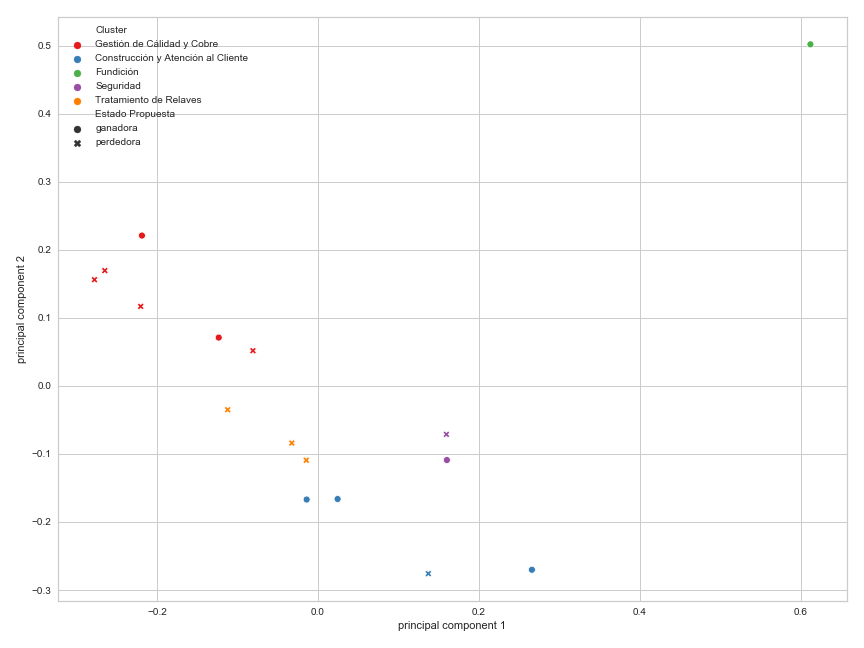
\includegraphics[width=1\textwidth]{figures/Clustering/PCA.png}
        \caption{\label{fig:PCA} Visualización de Clústers usando PCA} Fuente: Elaboración Propia.
    \end{figure}
    
    De la visualización, se pueden apreciar claramente las agrupaciones encontradas en nuestro proceso de \textit{clustering}. Además nuevamente, se puede ver cómo el documento que trata sobre Fundición es un outlier dentro de la muestra. 
    
\subsubsection{Opinión de Expertos}
    Una vez terminado todos los experimentos, se procedió a validar los resultados con un experto en el dominio. En nuestro caso se realizó una presentación a la Jefa de Desarrollo de Propuestas, persona líder del equipo encargado de compilar y validar una propuesta antes de ser enviada a los clientes de la compañía.
    
    A continuación se presentan cada uno de los puntos presentados y los respectivos comentarios sobre los resultados obtenidos:
    
    \begin{itemize}
        \item \textbf{Análisis mediante keywords}:
        \begin{itemize}
            \item Los conceptos comunes a cualquier propuesta detectados por el algoritmo, en general cumplen con los estándares que posee la compañía, por lo que son correctos. Por otro lado, los conceptos que destacan en propuestas ganadoras y no en perdedoras, interpretados por el analista como conceptos que podrían ayudar a una propuesta a ganar una licitación,  no entregan información tan valiosa. Esto ocurre ya que el análisis realizado no considera una segregación por clientes y en general las propuestas tienen un estándar distinto para cada uno de éstos. Otra segregación interesante que el análisis pasa por alto es el volumen de venta de una propuesta. En general existen distintos niveles de esfuerzo que se le dedican a las propuestas considerando el potencial volumen de venta que éstas podrían tener, por lo que repetir el experimento considerando esto también es algo que podría aumentar la calidad de la información detectada.
            
            \item Las conclusiones extraídas para algunos conceptos básicos, detectados por el analista, utilizando análisis de dispersión léxica son correctos en general. Por otro lado, se considera a la visualización como una buena herramienta de diagnóstico a una propuesta antes de ser enviada a un cliente. Esto debido a que las propuestas de Hatch hoy en día tienen un formato estandarizado para cada uno de los clientes, por lo que el gráfico de dispersión léxica debería ser el mismo para propuestas escritas para proyectos similares e iguales clientes. 
        \end{itemize}
        \item \textbf{Modelamiento de Tópicos }
        \begin{itemize}
            \item Los temas encontrados en el conjunto de propuestas analizados son correctos. Por otro lado, considerar que uno de los temas más relevantes en las propuestas analizadas es la Gestión de Calidad es coherente con los documentos revisados.
            \item Muchas de las conclusiones extraídas no son generalizables para todas las propuestas.
        \end{itemize}
        \item \textbf{Clustering}
        \begin{itemize}
            \item La información encontrada para el cliente Codelco división Chuquicamata, es considerada información valiosa que no había sido detectada.
        \end{itemize}
    \end{itemize}
    En general, se sugiere repetir los experimentos utilizando una mayor cantidad de datos y realizando los mismos análisis considerando una segregación por clientes y volumen de venta.
\subsubsection{Desarrollo de Guía}
    Considerando todos los patrones encontrados por el analista, más la opinión de los expertos. Se logró generar la siguiente guía de buenas prácticas para la construcción de propuestas técnicas en la compañía.
    \begin{itemize}
        \item Toda propuesta debe poseer al menos un apartado de Gestión de Calidad y otro de Seguridad.
        \item Relacionar los conceptos calidad y Hatch dentro de una misma oración en general tiene una buena acogida por parte de los clientes. Por otro lado, hablar sobre la relación que posee la compañía con los clientes durante el proyecto también es bien recibido.
        \item Se debe intentar hablar sobre las prácticas que posee la compañía sobre ciertos procesos genéricos dentro de un proyecto.
        \item Si la propuesta se está escribiendo para el cliente ``Codelco División Chuquicamata'', en general se debe hablar más sobre los aspectos técnicos de ésta por sobre los servicios extras que entrega Hatch tales como Post-Venta.
    \end{itemize}
